\title{Лекция 2\\Базовый язык представления знаний}   
\author[]{Шункевич Д.В.}
\institute[]{Белорусский государственный университет информатики и радиоэлектроники}

\begin{frame}
	\titlepage
\end{frame}

\begin{frame}{\\Содержание лекции}
	\topline
	\justifying
	Основные положения базового языка представления знаний в интеллектуальных системах – SC-кода.
	Алфавит, синтаксис, базовая денотационная семантика SC-кода.
	Синтаксическая и семантическая классификация sc-элементов.
\end{frame}

\begin{frame}{\\Архитектура фон-Неймана}
	\topline
	\justifying
	\vspace{10mm}
	\begin{figure}[H]
		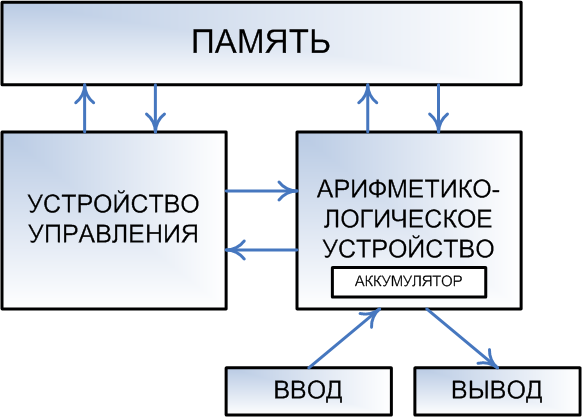
\includegraphics[scale=0.6]{./figures/sd_sc_code/neuman.png}
	\end{figure}
\end{frame}

\begin{frame}{\\Архитектура фон-Неймана}
	\topline
	\justifying
	\large
	\begin{textitemize}
		\item память ЭВМ однородна (линейна)
		\item доступ к ячейкам памяти ЭВМ осуществляется по адресу
		\item алфавитом, используемым для представления данных и команд, является множество {0, 1}
		\item каждая программа состоит из набора команд, выполняемых процессором последовательно
		\item возможно присутствие в программах команд условных переходов
	\end{textitemize}
\end{frame}

\begin{frame}{\\Двоичное представление}
	\topline
	\justifying
	\begin{columns}[T,onlytextwidth]
	\begin{column}{0.6\textwidth}
		\vspace{10mm}
		\begin{figure}[H]
			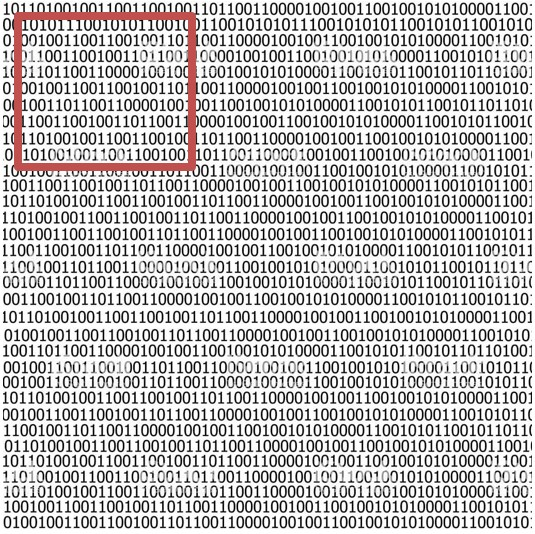
\includegraphics[scale=0.5]{./figures/sd_sc_code/binary.jpg}
		\end{figure}		
	\end{column}

	\begin{column}{0.4\textwidth}
	\vspace{10mm}
	\textbf{Достоинства:}
	\begin{textitemize}		
		\item легко реализовать
		\item удобно для машины
	\end{textitemize}		

	\bigskip
	\textbf{Недостатки:}
		
	\begin{textitemize}		
		\item неудобно для человека
		\item невозможно интерпретировать без контекста
	\end{textitemize}	

	\end{column}
\end{columns}
\end{frame}

\begin{frame}{\\Предлагаемый подход}
	\topline
	\justifying
	\large
	Разработать способ кодирования информации, который
	
	\begin{textitemize}
		\item удобен для представления и обработки в компьютере
		\item удобен для восприятия человеком
		\item обладает <<осмысленностью>>, может быть однозначно интерпретирован		
	\end{textitemize}

	\bigskip
	Требуется переход от \textit{данных} к \textit{знаниям}.

	\bigskip
	Одна из ключевых отличительных особенностей знаний\\ -- \uline{интерпретируемость} (Д. А. Поспелов).

\end{frame}

\begin{frame}{\\SC-code}
	\topline
	\justifying
	\begin{SCn}
		\scnheader{SC-code} 
		\scnidtf{способ универсального смыслового представления (кодирования) информации в памяти компьютерных систем}
		\scnidtf{semantic computer code}
		\scntext{примечание}{SC-code основан на \underline{теории графов} (синтаксис) и \underline{теории множеств} (семантика), что обеспечивает универсальность и унифицированность (единообразие) представления информации, удобство машинной обработки и восприятия человеком}
	\end{SCn}
\end{frame}

\begin{frame}{\\Сравнение SC-code и двоичного кодирования}
	\topline
	\justifying
	\vspace{10mm}
	\begin{textitemize}
		\item \textbf{Двоичное кодирование}
			\begin{textitemize}
				\item {алфавит \{0, 1\}}
				\item {не удобен для человека}
				\item {удобен для обработки в компьютере}
				\item {нельзя понять информацию без контекста}
				\item {легко реализовать}
			\end{textitemize}
		\item \textbf{\textit{SC-code}}
			\begin{textitemize}
				\item {базовый алфавит состоит из 5 элементов}
				\item {удобен для человека}
				\item {удобен для обработки в компьютере}
				\item {обладает «осмысленностью»}
			\end{textitemize}
		\end{textitemize}
\end{frame}

\begin{frame}{\\Формы представления SC-кода}
	\topline
	\justifying
	\vspace{10mm}
	\begin{SCn}
		\scnheader{SC-code}
		\scnidtf{абстрактный язык, который находится в памяти компьютерной системы}
		\scntext{примечание}{С помощью SC-кода можно описывать базы знаний, решатели задач и интерфейс интеллектуальной системы. SC-code является абстрактным языком, но его можно визуализировать в различных формах}
		\vspace{5mm}
		\textbf{Формы внешнего представления SC-кода}
			\begin{textitemize}
				\item {SCs-code (текстовый линейный)}
				\item {SCn-code (гипертекстовый)}
				\item {SCg-code (графический)}
			\end{textitemize}
	\end{SCn}
\end{frame}

\begin{frame}{\\Формы представления SC-кода}
	\topline
	\justifying
	\begin{columns}[T,onlytextwidth]
		\begin{column}{0.4\textwidth}
				\begin{SCn}
					\scnheader{SCs}
					\scnidtf{Semantic Code string}
					\scnidtf{язык линейного представления знаний}
					\scnheader{SCn}
					\scnidtf{Semantic Code natural}
					\scnidtf{язык структурированного представления знаний}
					\scnheader{SCg}
					\scnidtf{Semantic Code graphic}
					\scnidtf{язык графического представления знаний}
				\end{SCn}
		\end{column}
		\begin{column}{0.5\textwidth}
			\vspace{10mm}
			\begin{figure}[H]
				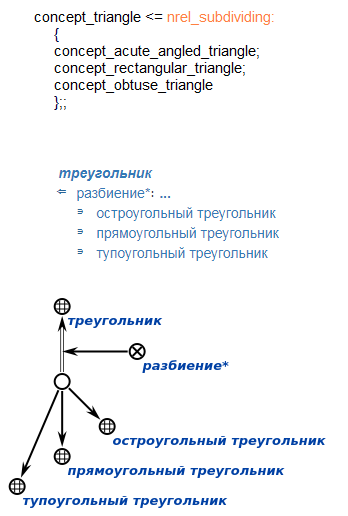
\includegraphics[scale=0.3]{./figures/sd_sc_code/ostis-basics-1.png}
			\end{figure}
		\end{column}
	\end{columns}
\end{frame}

\begin{frame}{\\Основные положения SC-кода}
	\topline
	\justifying
	\vspace{8mm}
	\begin{SCn}
		\scnheader{SC-код}
		\scntext{пояснение}{Информация содержится не в самих знаках, а в конфигурации связей между ними}
		\scniselement{абстрактный язык}
		\scniselement{графовый язык}
		\begin{scnrelfromset}{основные положения}
			\scnfileitem{знаки сущностей --  синтаксически элементарные фрагменты sc-текстов, такие знаки не имеют внутренней структуры}
			\scnfileitem{информационные конструкции, не являющиеся sc-текстами, могут быть включены в базу знаний в виде файлов}
			\scnfileitem{тексты sc-кода имеют нелинейную структуру, так как каждый знак сущности входит в базу знаний однократно и имеет неограниченное количество связей с другими знаками сущностей}
		\end{scnrelfromset}
	\end{SCn}
\end{frame}

\begin{frame}{\\}
	\topline
	\justifying
	\begin{SCn}
		\scnheader{SC-код}
		\begin{scnrelfromset}{основные положения}
			\scnfileitem{база знаний является графовой структурой, алфавит элементов которой включает в себя множество узлов, рёбер, дуг, базовых дуг, а также множество специальных узлов (файлов)}
			\scnfileitem{структурная особенность графовой структуры базы знаний заключается в том, что её дуги и ребра могут связывать не только узел с узлом, но и узел с ребром или дугой и т.д.}
			\scnfileitem{отсутствие синонимии осуществляется благодаря склеиванию одинаковых sc-элементов}
			\scnfileitem{sc-узлы, sc-ребра и sc-дуги являются обозначениями различных сущностей}
		\end{scnrelfromset}
	\end{SCn}
\end{frame}

\begin{frame}{\\Cинтаксис. Алфавит SC-кода}
	\topline
	\justifying
	\begin{SCn}
		\scnheader{алфавит SC-кода}
		\scnidtf{семейство синтаксических меток, приписываемых sc-элементам и указывающих факт принадлежности sc-элемента к соответствующему классу sc-элементов}
		
		\scnheader{минимальный алфавит SC-кода}
		\scntext{пояснение}{Для понимания sc-конструкций, хранимых в sc-памяти, достаточно синтаксически выделить только \textit{Класс константных постоянных позитивных sc-пар принадлежности (Класс базовых sc-дуг)}, с помощью которых каждый sc-элемент будет явно соединяться с sc-классами, которым этот sc-элемент принадлежит. Очевидно, что таким явным способом выделить базовые sc-дуги с помощью самих этих базовых sc-дуг невозможно.}
	\end{SCn}
\end{frame}

\begin{frame}{\\Минимальный алфавит SC-кода}
	\topline
	\justifying
	\begin{SCn}
		Таким образом, любой класс sc-элементов можно выделить явно путём:\\
		\begin{textitemize}
			\item{введения sc-элемента, являющегося знаком этого класса sc-элементов (sc-класса);}
			\item{проведения постоянных позитивных sc-пар принадлежности во все sc-элементы, являющиеся элементами
			выделяемого sc-класса и хранимые (присутствующие) в текущем состоянии sc-памяти.}
		\end{textitemize}
	
		\scnheader{минимальный алфавит SC-кода}
		\scnidtf{\textit{Класс базовых sc-дуг} и \textit{Класс всех остальных sc-элементов} (по умолчанию)}
	\end{SCn}
\end{frame}

\begin{frame}{\\Алфавит Ядра SC-кода}
	\topline
	\justifying
	\begin{SCn}
		\begin{columns}[T,onlytextwidth]
			\begin{column}{0.7\textwidth}
				\vspace{5mm}
				\scnheader{Алфавит Ядра SC-кода}
				\begin{scneqtoset}
					\scnitem{sc-узел, являющийся знаком файла}
					\scnitem{sc-узел, не являющийся знаком файла}
					\scnitem{базовая sc-дуга}
					\scnitem{sc-ребро}
					\scnitem{sc-дуга общего вида}
				\end{scneqtoset}
			\end{column}
			\begin{column}{0.3\textwidth}
				\begin{figure}[H]
					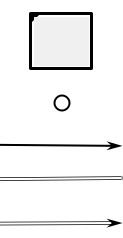
\includegraphics[scale=0.7]{./figures/sd_sc_code/abc.png}
				\end{figure}
			\end{column}
		\end{columns}
	\end{SCn}
\end{frame}

\begin{frame}{\\Алфавит Ядра SC-кода}
	\topline
	\justifying
	\begin{SCn}
	\vspace{10mm}
		
	\scriptsize
	
	\scnheader{sc-ребро}
	\scnidtf{Класс \textit{sc-элементов}, имеющих в рамках \textit{Ядра SC-кода} синтаксическую метку \textit{обозначений неориентированных sc-пар}}
	
	\scnheader{sc-дуга общего вида}
	\scnidtf{Класс \textit{sc-элементов}, имеющих в рамках \textit{Ядра SC-кода} синтаксическую метку \textit{обозначений ориентированных sc-пар, не являющихся постоянными позитивными sc-парами принадлежности}}
	
	\scnheader{базовая sc-дуга}
	\scnidtf{Класс \textit{sc-элементов}, имеющих в рамках \textit{Ядра SC-кода} синтаксическую метку \textit{постоянных позитивных sc-пар принадлежности}}
	
	\scnheader{sc-узел, являющийся знаком файла}
	\scnidtf{\textit{sc-элементов}, имеющий в рамках \textit{Ядра SC-кода} синтаксическую метку \textit{sc-элементов}, являющихся знаками \textit{файлов}}
	
	\scnheader{sc-узел, не являющийся знаком файла}
	\scnidtf{\textit{sc-узел}, имеющий в рамках \textit{Ядра SC-кода} синтаксическую метку \textit{sc-элементов, не являющихся ни знаками файлов, ни обозначениями sc-пар}}
	\end{SCn}
\end{frame}

\begin{frame}{\\Семантическая классификация sc-элементов}
	\topline
	\justifying 
	\textbf{}\\
	К числу базовых признаков классификации \textit{sc-элементов} относятся:
	\begin{textitemize}
		\item структурный признак;
		\item логико-семантический признак;
		\item темпоральная характеристика сущностей, обозначаемых sc - элементами, которая в свою очередь, включает в себя:
		\begin{textitemize}
			\item постоянство или временность существования обозначаемой сущности;
			\item статичность (стационарность) или динамичность (изменчивость) обозначаемой сущности.
		\end{textitemize}
	\end{textitemize}
\end{frame}

\begin{frame}{\\Структурная классификация sc-элементов}
	\topline
	\justifying 
	\vspace{10mm}
	\begin{SCn}
		\scnheader{sc-элемент}
		\scnrelfrom{разбиение}{Структурный признак классификации sc-элементов}
		\begin{scnindent}
			\begin{scneqtoset}
				\scnitem{обозначение sc-множества}
				\scnitem{обозначение внешней сущности}
				\begin{scnindent}
					\begin{scnrelfromset}{разбиение}
						\scnitem{обозначение файла}
						\scnitem{обозначение информационной конструкции, не являющейся ни sc-множеством, ни файлом}
						\scnitem{обозначение внешней сущности, не являющейся информационной конструкцией}
					\end{scnrelfromset}
				\end{scnindent}
			\end{scneqtoset}
		\end{scnindent} 
	\end{SCn}
\end{frame}

\begin{frame}{\\Структурная классификация sc-элементов}
	\topline
	\justifying 
	\vspace{3mm}
	\footnotesize
	\begin{SCn}
		\scnheader{обозначение sc-множества}
			\begin{scnrelfromset}{разбиение}
			\scnitem{обозначение sc-связки}
				\begin{scnindent}
				\begin{scnrelfromset}{разбиение}
					\scnitem{обозначение sc-синглетона}
					\scnitem{обозначение sc-пары}
						\begin{scnindent}
						\begin{scnrelfromset}{разбиение}
							\scnitem{обозначение неориентированной sc-пары}
							\scnitem{обозначение ориентированной sc-пары}
						\end{scnrelfromset}
						\end{scnindent}
					\scnitem{обозначение sc-связки, не являющейся синглетоном и парой}
				\end{scnrelfromset}
				\end{scnindent}
			\scnitem{обозначение sc-класса}
			\scnitem{обозначение sc-структуры}
		\end{scnrelfromset}
	\end{SCn}
\end{frame}

\begin{frame}{\\}
	\topline
	\justifying 
	\begin{SCn}
		\scnheader{обозначение ориентированной sc-пары}
		\begin{scnrelfromset}{разбиение}
			\scnitem{обозначение sc-пары принадлежности}
			\begin{scnindent}
				\begin{scnrelfromset}{разбиение}
					\scnitem{обозначение sc-пары нечеткой принадлежности}
					\scnitem{обозначение sc-пары позитивной принадлежности}
					\scnitem{обозначение sc-пары негативной принадлежности}
				\end{scnrelfromset}
			\end{scnindent}
			\scnitem{обозначение ориентированной sc-пары, не являющейся парой принадлежности}
		\end{scnrelfromset}
	\end{SCn}
\end{frame}

\begin{frame}{\\Логико-семантическая классификация}
	\topline
	\justifying 
	\begin{SCn}
		\scnheader{Логико-семантическая классификация sc-элементов}
		\scnstartstruct
		\scnheader{sc-элемент}
			\begin{scnrelfromset}{разбиение}
				\scnitem{sc-константа}
					\begin{scnindent}
						\scnidtf{sc-элемент, логико-семантическим значением которого является он сам}
					\end{scnindent}
				\scnitem{sc-переменная}
			\end{scnrelfromset}	
	\scnendstruct 
	\end{SCn}
\end{frame}

\begin{frame}{\\}%Возможно лишнее
	\topline
	\justifying 
	\begin{SCn}
		\scnheader{Классификация sc-элементов по темпоральным характеристикам обозначаемых ими сущностей}
		\scnstartstruct
		\scnheader{sc-элемент}
		\scnrelfrom{разбиение}{Признак постоянства существования сущностей, обозначаемых sc-элементами}
			\begin{scnindent}
				\begin{scneqtoset}
					\scnitem{обозначение постоянной сущности}
					\begin{scnindent}
						\scnidtf{обозначение постоянно существующей сущности}
					\end{scnindent}
					\scnitem{обозначение временной сущности}
				\end{scneqtoset}
			\end{scnindent} 
		\scnendstruct 
	\end{SCn}
\end{frame}

\begin{frame}{\\Признак статичности сущностей}%Возможно лишнее
	\topline
	\justifying 
	\begin{SCn}
		\scnheader{sc-элемент}
		\scnrelfrom{разбиение}{Признак статичности сущностей, обозначаемых sc-элементами}
		\begin{scnindent}
			\begin{scneqtoset}
				\scnitem{обозначение статической сущности}
				\begin{scnindent}
					\scnidtf{обозначение сущности, изменения которой в рамках соответствующего отрезка времени считаются несущественными}
					\scnsuperset{обозначение статического sc-множества}
				\end{scnindent}
				\scnitem{обозначение динамической сущности}
				\begin{scnindent}
					\scnidtf{обозначение сущности изменяющейся во времени}
					\scnsuperset{обозначение динамического sc-множества}
				\end{scnindent}
			\end{scneqtoset}
		\end{scnindent} 
	\end{SCn}
\end{frame}

\begin{frame}{\\Обозначение временной сущности}%Возможно лишнее
	\topline
	\justifying 
	\begin{SCn}
	\scnheader{обозначение временной сущности}
		\begin{scnrelfromset}{разбиение}
			\scnitem{обозначение внешней временной сущности}
			\begin{scnindent}
				\scnsuperset{обозначение внешней ситуации}
				\scnsuperset{обозначение внешнего события}
				\scnsuperset{обозначение внешнего процесса}
			\end{scnindent}
			\scnitem{обозначение внутренней временной сущности в sc-памяти}
		\end{scnrelfromset}
	\end{SCn}
\end{frame}

\begin{frame}{\\}%Возможно лишнее
	\topline
	\justifying 
	\begin{SCn}
		\scnheader{обозначение внутренней временной сущности в sc-памяти}
			\begin{scnrelfromset}{разбиение}
				\scnitem{обозначение ситуации в sc-памяти}
				\begin{scnindent}
					\scnidtf{обозначение ситуации, которая возникла или возникает в процессе обработки информации в sc-памяти}
				\end{scnindent}
				\scnitem{обозначение события в sc-памяти}
				\begin{scnindent}
					\scnidtf{обозначение события, которое произошло или произойдет в процессе обработки информации в sc-памяти}
				\end{scnindent}
				\scnitem{обозначение информационного процесса в sc-памяти}
				\begin{scnindent}
					\scnidtf{обозначение внутреннего процесса в sc-памяти, который происходит, произошёл или будет происходить}
				\end{scnindent}
			\end{scnrelfromset}
	\end{SCn}
\end{frame}

\begin{frame}{\\Темпоральные свойства sc-элементов}%Возможно лишнее
	\topline
	\justifying 
	\vspace{10mm}
	\begin{SCn}
		\textbf{Когда речь идёт о темпоральных свойствах sc-элементов, следует чётко отличать:}
		\begin{textitemize}
			\item временный характер присутствия любого sc-элемента в составе той базы знаний, в которой он находится 
			\item временный характер присутствия в sc-памяти всей заданной sc-конструкции  (ситуации в sc-памяти);
			\item временный характер существования внешней сущности, которую sc-элемент обозначает;
			\item статичный (динам.) характер внешней сущности, обозначаемой sc-элементом; динамический характер внешней сущности, предполагает наличие в sc-памяти описания процесса изменения состояния или конфигурации указанной внешней сущности;
			\item динам. sc-множество, являющееся отражением соответствующего внешнего процесса;
			\item динам. sc-множество, являющееся отражением  соответствующего внутреннего процесса 
		\end{textitemize}
	\end{SCn}
\end{frame}

\begin{frame}{\\Структурная классификация sc-констант}
	\topline
	\justifying 
	\begin{SCn}
			Данная классификация полностью аналогична \textit{Структурной классификации sc-элементов}, в отличие от которой она описывает структурную классификацию только константных sc-элементов (sc-констант)
	\end{SCn}
\end{frame}

\begin{frame}{\\Структурная классификация sc-констант}
	\topline
	\justifying 
	\begin{SCn}
		\scnheader{Структурная классификация sc-констант}
		\scnstartstruct
		\scnheader{sc-константа}
		\begin{scnrelfromset}{разбиение}
			\scnitem{sc-множество}
			\scnitem{внешняя сущность}
		\end{scnrelfromset}
		
	\scnendstruct
	\end{SCn}
\end{frame}

\begin{frame}{\\внешняя сущность}
	\topline
	\justifying 
	\begin{SCn}
		\scnheader{внешняя сущность}
		\scnidtf{sc-элемент, являющийся знаком внешней сущности}
		\scnidtf{знак внешней сущности}
		\scnidtf{знак сущности, не являющейся sc-множеством (sc-конструкцией)}
		\begin{scnrelfromset}{разбиение}
			\scnitem{файл}
			\scnitem{внутренний файл}
			\scnitem{внешняя сущность, не являющаяся внутренним файлом}
			\scnitem{внешняя сущность, не являющаяся информационной конструкцией}
			\scnitem{информационная конструкция, не являющаяся ни sc-множеством, ни файлом}
		\end{scnrelfromset}
	\end{SCn}
\end{frame}

\begin{frame}{\\sc-множество}
	\topline
	\justifying 
	\begin{SCn}
		\scnheader{sc-множество}
			\begin{scnindent}
			\begin{scnrelfromset}{разбиение}
				\scnitem{sc-связка}
					\begin{scnindent}
					\begin{scnrelfromset}{разбиение}
						\scnitem{sc-синглетон}
						\scnitem{sc-пара}
						\scnitem{sc-связка, не являющаяся синглетоном и парой}
					\end{scnrelfromset}
					\end{scnindent}
				\scnitem{sc-класс}
				\scnitem{sc-структура}
			\end{scnrelfromset}
			\end{scnindent}
	\end{SCn}
\end{frame}

\begin{frame}{\\sc-пара}
	\topline
	\justifying 
	\vspace{5mm}
	\begin{SCn}
		\scnheader{sc-пара}
		\begin{scnrelfromset}{разбиение}
			\scnitem{неориентированная sc-пара}
			\scnitem{ориентированная sc-пара}
				\begin{scnindent}
				\begin{scnrelfromset}{разбиение}
					\scnitem{sc-пара принадлежности}
						\begin{scnindent}
						\begin{scnrelfromset}{разбиение}
							\scnitem{sc-пара нечёткой принадлежности}
							\scnitem{sc-пара позитивной принадлежности}
							\scnitem{sc-пара негативной принадлежности}
						\end{scnrelfromset}
						\end{scnindent}
					\scnitem{ориентированнная sc-пара, не являющаяся sc-парой принадлежности}	
				\end{scnrelfromset}
				\end{scnindent}
		\end{scnrelfromset}
	\end{SCn}
\end{frame}

\begin{frame}{\\sc-пара позитивной принадлежности}
	\topline
	\justifying 
	\vspace{5mm}
	\begin{SCn}
		\scnheader{sc-пара позитивной принадлежности}	
		\scnsuperset{sc-пара постоянной позитивной принадлежности}
			\begin{scnindent}
			\begin{scnreltoset}{пересечение множеств}
				\scnitem{sc-константа}
				\scnitem{постоянная сущность}
				\scnitem{статическая сущность}
				\scnitem{sc-пара позитивной принадлежности}	
			\end{scnreltoset}
			\end{scnindent}
		\scnsuperset{sc-пара временной позитивной принадлежности}
			\begin{scnindent}
			\begin{scnreltoset}{пересечение множеств}
				\scnitem{sc-константа}
				\scnitem{временная сущность}
				\scnitem{динамическая сущность}
				\scnitem{sc-пара позитивной принадлежности}	
			\end{scnreltoset}
			\end{scnindent}
	\end{SCn}
\end{frame}
